% ============================================================================
%  Does Financial News Sentiment Improve Neural-SDE Option Pricing?
%  Compile:  pdflatex main.tex   (twice, for cross-references)
%  Figures expected in ./figures/ — see \graphicspath below.
% ============================================================================
\documentclass[11pt,a4paper]{article}

\usepackage[utf8]{inputenc}
\usepackage[T1]{fontenc}
\usepackage{amsmath,amssymb}
\usepackage{booktabs}
\usepackage{graphicx}
\usepackage{geometry}
\usepackage{natbib}
\usepackage{hyperref}
\usepackage{caption}
\usepackage{longtable}

\geometry{margin=1in}
\graphicspath{{figures/}{figures/paper/}}
\hypersetup{colorlinks=true,linkcolor=blue,citecolor=blue,urlcolor=blue}
\bibliographystyle{plainnat}

\title{Does Financial News Sentiment Improve Neural-SDE Option Pricing?\\
       Evidence from a Corrected Two-Stage Calibration Pipeline}

\author{Ethan Itkis \and Matthew Lascoe \and Stephen Linehan-Reckford \and
        Om Patel \and Samuel Shlyam\\[4pt]
        \small Stevens Institute of Technology}

\date{\today}

\begin{document}
\maketitle

\begin{abstract}
We test whether daily financial-news sentiment, extracted from Refinitiv/LSEG
news via FinBERT, improves the pricing accuracy of neural stochastic-volatility
models calibrated to S\&P~500 index options. Following the two-stage
deep-calibration framework of \citet{horvath2021}, we pre-train a convolutional
network offline on synthetic implied-volatility surfaces generated from four
stochastic-volatility families---Heston, Bates, one-factor Bergomi and rough
Bergomi---and then fine-tune it online against historical SPX surfaces through a
fully differentiable pricer. Two arms are compared under identical architecture
and hyperparameters: a baseline that sees only the implied-volatility surface,
and a sentiment arm that additionally receives a daily sentiment channel. We
evaluate 32 (model, regime, arm) cells across four market regimes spanning
2010--2022.

Offline, the sentiment channel is genuinely informative: the sentiment arm
attains 4--25\% lower validation loss than the baseline across all four model
families. Online, the picture is far more equivocal. In-sample,
Diebold-Mariano tests find statistically significant differences in 11 of 16
cells, but split 7 favourable and 4 unfavourable with effect sizes below 5\%.
Under expanding-window walk-forward evaluation---the more demanding test---7
cells favour sentiment and 6 favour the baseline, and the in-sample and
out-of-sample verdicts disagree in 6 of 16 cells. The largest in-sample
sentiment advantage (Heston, 2010--2012, DM $t=12.46$) vanishes out-of-sample
($t=-0.44$), while Bates reverses from in-sample unfavourable to out-of-sample
favourable in three regimes. Robust, sign-consistent sentiment gains survive in
only a minority of cells. All findings are reported with Benjamini-Hochberg
control of the false discovery rate.

Two further findings bound any interpretation. First, a previous-day persistence
forecast attains lower surface error than every calibrated variant in all 16
cells under the vega-weighted implied-volatility metric, by a mean factor of
2.0---but the same comparison in price space yields a mean ratio of only 1.08,
and a converged classical least-squares calibration of the same pricer attains
comparable accuracy. The choice of error metric, not the calibration method,
drives the apparent dominance of the naive benchmark. Second, an identification
analysis shows that most structural parameters are only weakly recovered, and
the sentiment channel does not improve identification.
\end{abstract}

\noindent\textbf{Keywords:} deep calibration; stochastic volatility; implied
volatility surface; FinBERT; sentiment analysis; walk-forward evaluation

\vspace{1em}
\noindent\textbf{JEL:} C45, C58, G13

\section{Introduction}

\subsection{Motivation}
Deep calibration has made parametric stochastic-volatility models tractable at
speeds classical optimisation cannot approach. By learning the map from implied
volatility surfaces to model parameters offline, a neural network replaces a
costly inner optimisation loop with a single forward pass
\citep{horvath2021,bayer2018}. This opens a question that was previously
impractical to ask: if the calibration network can absorb an arbitrary input
channel at negligible cost, can it exploit information beyond the surface itself?

Financial news sentiment is a natural candidate. A substantial literature links
investor sentiment to returns and to the cross-section of asset prices
\citep{baker2006,tetlock2007}. If sentiment carries information about the
risk-neutral density that the current surface has not yet fully impounded, a
calibration network given both should outperform one given only the surface.

\subsection{Research question}
What is the effect of supplying a daily financial-news sentiment signal to the
training and calibration of a neural stochastic-differential-equation
option-pricing model, and does that effect survive out-of-sample evaluation?

\subsection{Contributions}
\begin{enumerate}
\item We construct a two-arm experiment in which the sentiment and baseline
models are identical in architecture, hyperparameters, data and random seeds,
differing only in the presence of a sentiment input channel.
\item We evaluate the arms not only on in-sample surface fit but under
expanding-window walk-forward calibration, and show that the two disagree in 6
of 16 cells---including cases where the strongest in-sample effect disappears
entirely.
\item We benchmark both arms against a previous-day persistence forecast and
find that neither beats it in any cell under the standard vega-weighted
implied-volatility metric.
\item We show that this benchmark comparison reverses in magnitude depending on
whether error is measured in implied-volatility or price units, and that a
converged classical least-squares calibration of the same pricer attains
comparable accuracy---locating the residual error in the model class rather than
in the calibration method.
\item We document and correct seven data-generation defects in the offline stage
that, left in place, produce qualitatively different and misleading conclusions
(Appendix~\ref{app:corrections}).
\end{enumerate}

\subsection{Hypotheses}
The study was designed around two pre-registered hypotheses:
\begin{description}
\item[H1 (pricing).] The sentiment arm attains lower surface pricing error than
the baseline, with the largest improvements in high-volatility regimes.
\item[H2 (hedging).] The sentiment arm attains lower delta-hedged
profit-and-loss variance than the baseline.
\end{description}
All other analyses are exploratory and are labelled as such.

\section{Related work}

\paragraph{Deep calibration.} Neural approximation of pricing maps dates to
\citet{hutchinson1994}, but the modern two-stage form is due to
\citet{horvath2021}, with related contributions by \citet{bayer2018} and
\citet{ferguson2018}.

\paragraph{Stochastic volatility.} We evaluate four families:
\citet{heston1993}, its jump extension \citet{bates1996}, the one-factor
forward-variance model of \citet{bergomi2005}, and rough Bergomi
\citep{bayer2016}. The last reflects evidence that volatility is rough, with
Hurst exponents well below $1/2$ \citep{gatheral2018}. \citet{bakshi1997}
remains the reference point for comparative empirical performance.

\paragraph{Sentiment.} We use FinBERT \citep{araci2019}, a BERT variant
\citep{devlin2019} fine-tuned for financial text, following the finding that
domain-specific lexicons outperform general-purpose ones in finance
\citep{loughran2011}. Whether news tone carries pricing-relevant information
beyond price history goes back at least to \citet{tetlock2007}.

\paragraph{Surface dynamics.} Our persistence-benchmark finding connects to work
on the predictable dynamics of the implied volatility surface
\citep{goncalves2006,cont2002}.

\section{Data}

\subsection{Option data}
We use daily S\&P~500 index option quotes partitioned into four regimes:

\begin{table}[h]
\centering
\begin{tabular}{llr}
\toprule
Regime & Character & Trading days \\
\midrule
2010--2012 & Post-crisis recovery & 744 \\
2013--2015 & Low-volatility expansion & 727 \\
2016--2019 & Extended calm, four years & 995 \\
2020--2022 & COVID shock and aftermath & 749 \\
\bottomrule
\end{tabular}
\end{table}

For each trade date we build an $8\times11$ grid of 8 maturity slices,
$\tau \in \{0.1,0.3,0.6,0.9,1.2,1.5,1.8,2.0\}$ years, by 11 log-moneyness levels
spanning $[-0.5,+0.5]$. Days with insufficient coverage are dropped.

\subsection{Forward reconstruction and normalisation}
Option prices are normalised by the forward rather than by a spot proxy.
Discount factors are built from FRED Treasury yields (DGS1MO--DGS3Y)
interpolated to each option's maturity, with a constant 1.9\% dividend yield.
Working in forward units removes the dividend yield from the pricing map, since
the forward is by construction the martingale numeraire.

We replace the percentile-based global price cap used in earlier iterations with
a no-arbitrage band filter that drops quotes outside $[\text{intrinsic},
\text{forward}]$. The band filter removes 0.28\% of rows; after filtering, 100\%
of retained prices are invertible to implied volatility, with a median shift of
$-0.0017$ volatility points relative to the vendor's own implied volatilities.

\subsection{News sentiment}
Article-level sentiment is extracted with FinBERT from Refinitiv/LSEG Machine
Readable News, filtered to U.S. equity-market relevance. The corpus spans
4~January~2010 to 31~January~2025 and comprises \textbf{227{,}424 articles
across 3{,}794 trading days}, a mean of 59.9 and median of 50 articles per day
(maximum 422). Articles are split into 400-character chunks, yielding
\textbf{2{,}384{,}978 chunks}, an average of 10.5 per article.

FinBERT returns a probability distribution over positive, negative and neutral
for each chunk. Chunk probabilities are averaged within an article, and the
continuous article score is $P(\text{pos}) - P(\text{neg})$. Article scores are
averaged by publication date to yield a daily sentiment index.

The news corpus extends beyond the option sample; the evaluation period ends in
2022 because the regime partition is bounded by the option data.

\section{Synthetic data generation}

\subsection{Parameter sampling and surface construction}
For each family we sample 50{,}000 parameter vectors uniformly from the bounds
in Table~\ref{tab:bounds} and price the corresponding $8\times11$ surface, using
Fourier methods where a characteristic function is available \citep{carr1999}
and Monte Carlo otherwise.

\begin{table}[h]
\centering
\caption{Parameter sampling bounds. 50{,}000 vectors per family, uniform.}
\label{tab:bounds}
\begin{tabular}{lll}
\toprule
Family & Parameter & Range \\
\midrule
\textbf{Heston} & $\kappa$ mean-reversion speed & $[0.1,\ 3.0]$ \\
 & $\theta$ long-run variance & $[0.01,\ 0.15]$ \\
 & $\sigma$ vol-of-vol & $[0.1,\ 0.8]$ \\
 & $v_0$ initial variance & $[0.01,\ 0.15]$ \\
 & $\rho$ spot--variance correlation & $[-0.90,\ -0.10]$ \\
\midrule
\textbf{Bates} & $\kappa,\theta,\sigma,v_0,\rho$ & as Heston \\
 & $\lambda_J$ jump intensity & $[0,\ 2.0]$ \\
 & $\mu_J$ mean jump size & $[-0.20,\ 0.05]$ \\
 & $\sigma_J$ jump volatility & $[0.01,\ 0.20]$ \\
\midrule
\textbf{Bergomi} & $\xi$ initial forward variance & $[0.01,\ 0.16]$ \\
 & $\nu$ vol-of-vol & $[0.5,\ 4.0]$ \\
 & $\rho$ & $[-0.95,\ -0.10]$ \\
 & $\beta$ & $[0,\ 10.0]$ \\
\midrule
\textbf{rBergomi} & $\xi,\nu,\rho$ & as Bergomi \\
 & $H$ Hurst exponent & $[0.025,\ 0.50]$ \\
\bottomrule
\end{tabular}
\end{table}

The spot--variance correlation is sampled strictly negative in both families,
imposing the leverage effect as a structural restriction rather than leaving its
sign to be recovered. The mean jump size is likewise predominantly negative,
consistent with the downward-skewed jump risk priced into index options. The
Hurst exponent spans $[0.025, 0.50]$, covering the rough regime documented
empirically \citep{gatheral2018} up to the classical Brownian endpoint. These
bounds give the reference distribution for the identification analysis in
Section~\ref{sec:ident}.

Three properties of the generator warrant emphasis, because each was a defect in
an earlier iteration (Appendix~\ref{app:corrections}):
\begin{itemize}
\item \textbf{Martingale correction.} Simulated terminal prices are rescaled so
that $\mathbb{E}[S_T]$ matches the forward. Without it the discretised variance
process induces a drift error reaching $-19\%$ at $T=2$.
\item \textbf{Full truncation.} The variance process uses full truncation
\citep{lord2010} rather than naive clamping.
\item \textbf{Log-moneyness grid.} Synthetic surfaces use the same log-moneyness
grid as the market surfaces.
\end{itemize}
After correction, the fraction of synthetic surface points failing to invert
falls from 16.8--37.6\% to 0.22--0.70\%.

\subsection{Synthetic sentiment}
\label{sec:synthsent}

\paragraph{Endogenous sentiment-driven dynamics.}
Rather than generating price paths and attaching sentiment post hoc, the
simulation couples every path to a latent sentiment process. Sentiment $Y_t$
follows an Ornstein-Uhlenbeck process augmented with compound Poisson jumps,
\begin{equation}
dY_t = \kappa_Y(\theta_Y - Y_t)\,dt + \sigma_Y\,dW_t^Y + dJ_t^Y ,
\end{equation}
with parameters sampled independently per surface. This latent process enters
the variance dynamics multiplicatively,
\begin{equation}
dV_t = \kappa\bigl(\theta e^{\beta_V Y_t} - V_t\bigr)dt
       + \sigma\sqrt{V_t}\,dW_t^V ,
\end{equation}
and the log-price drift additively through $\beta_S Y_t$; its innovations are
correlated with the price shocks. Sentiment therefore has a structural, causal
effect on the simulated dynamics rather than being a label attached to an
independently generated surface.

Crucially, $Y_t$ is \emph{not} supplied to the network. To preserve a strict
analogy with the empirical setting---where FinBERT scores are an imperfect,
noisy observation of an unobservable market mood---we compute return-based path
statistics from the sentiment-driven trajectories and pass them through the
empirical regression below to produce the synthetic scores the network sees.

\paragraph{The empirical sentiment map.}
Because sentiment is bounded in $(-1,1)$, we model it in unbounded space: the
response is $y = \operatorname{arctanh}(s)$, mapped back through $\tanh$. The
predictors are computable from any price path. After the 21-day rolling-window
burn-in, $n = 3{,}774$ of the 3{,}794 available days enter the regression.

\begin{table}[h]
\centering
\caption{Regression of $\operatorname{arctanh}$-transformed daily FinBERT
sentiment on return-based path statistics. Residual s.e.\ 0.1122 on 3{,}762 d.f.
$R^2 = 0.5080$, adjusted $R^2 = 0.5065$, $n = 3{,}774$. In sentiment space
$R^2 = 0.4979$.}
\label{tab:regression}
\begin{tabular}{lrrrr}
\toprule
Variable & Estimate & Std.\ Error & $t$ & $\Pr(>|t|)$ \\
\midrule
(Intercept)      & $0.06556$   & $0.00608$  & $10.783$  & $<2\times10^{-16}$ \\
y\_lag1          & $0.68555$   & $0.01170$  & $58.599$  & $<2\times10^{-16}$ \\
ret              & $-3.22856$  & $0.19308$  & $-16.721$ & $<2\times10^{-16}$ \\
ret\_sq          & $13.05354$  & $7.07931$  & $1.844$   & $0.0652$ \\
abs\_ret         & $-2.27957$  & $0.41895$  & $-5.441$  & $5.29\times10^{-8}$ \\
roll\_mean\_5    & $1.04134$   & $0.60250$  & $1.728$   & $0.0839$ \\
roll\_mean\_21   & $-6.59953$  & $2.54445$  & $-2.594$  & $0.0095$ \\
roll\_vol\_5     & $1.03807$   & $0.55849$  & $1.859$   & $0.0631$ \\
roll\_vol\_21    & $4.60709$   & $2.40796$  & $1.913$   & $0.0557$ \\
downside\_21     & $-5.99732$  & $3.11629$  & $-1.925$  & $0.0543$ \\
drawdown\_21     & $0.12228$   & $0.17800$  & $0.687$   & $0.4920$ \\
realized\_var\_21& $-10.62001$ & $15.99044$ & $-0.664$  & $0.5070$ \\
\bottomrule
\end{tabular}
\end{table}

The fit explains roughly half the variation in daily sentiment and is dominated
by persistence: lagged sentiment enters with coefficient 0.686 and $t = 58.6$.
The clearest market linkages are contemporaneous returns ($t = -16.7$) and
absolute returns ($t = -5.4$).

\paragraph{A limitation of this construction.} The dominant predictor, lagged
sentiment, has no analogue on a simulated path with no news history. The
generator substitutes a path-derived proxy (a $z$-scored lagged return). The
synthetic channel therefore reproduces the return-driven component of real
sentiment but not its autoregressive persistence.

\subsection{Channel representation}
The baseline arm receives a single-channel $8\times11$ implied-volatility grid.
The sentiment arm receives two channels: the surface, and a sentiment channel
broadcast across strikes within each maturity slice. The two arms are otherwise
identical. The sentiment channel is standardised per regime; the offline channel
has pooled mean $-0.0296$ and standard deviation $0.0927$, and the resulting
per-regime scale factors are 0.647, 0.917, 0.790 and 0.863.

\section{Method}

\subsection{Offline pre-training}
A convolutional network maps the input surface to the parameter vector: 2-D
convolutions with batch normalisation and ELU activations, a dense head with
dropout, a sigmoid output, and a scaling layer mapping to each parameter's
admissible range. Training minimises error against the known generating
parameters using Adam with a ReduceLROnPlateau schedule.

\begin{table}[h]
\centering
\caption{Offline pre-training, best validation loss.}
\label{tab:offline}
\begin{tabular}{lrrr}
\toprule
Model & Baseline (In1) & Sentiment (In2) & Improvement \\
\midrule
Heston   & 0.00349 & 0.00261 & 25\% \\
Bates    & 0.01213 & 0.01123 & 7\% \\
Bergomi  & 0.00336 & 0.00322 & 4\% \\
rBergomi & 0.00347 & 0.00321 & 7\% \\
\bottomrule
\end{tabular}
\end{table}

The sentiment arm attains lower validation loss in every family, establishing
that the channel is learnable. Whether that capability transfers to real
sentiment is the question the online stage answers.

\subsection{Online fine-tuning}
The pre-trained weights initialise an unsupervised refinement loop against
market surfaces. The network predicts parameters; a differentiable pricer prices
the $8\times11$ grid; and the reconstruction error is backpropagated through the
pricer into the network. The objective is Huber loss on the surface. Each of the
32 cells is fine-tuned independently for 750 epochs.

\begin{figure}[h]
\centering
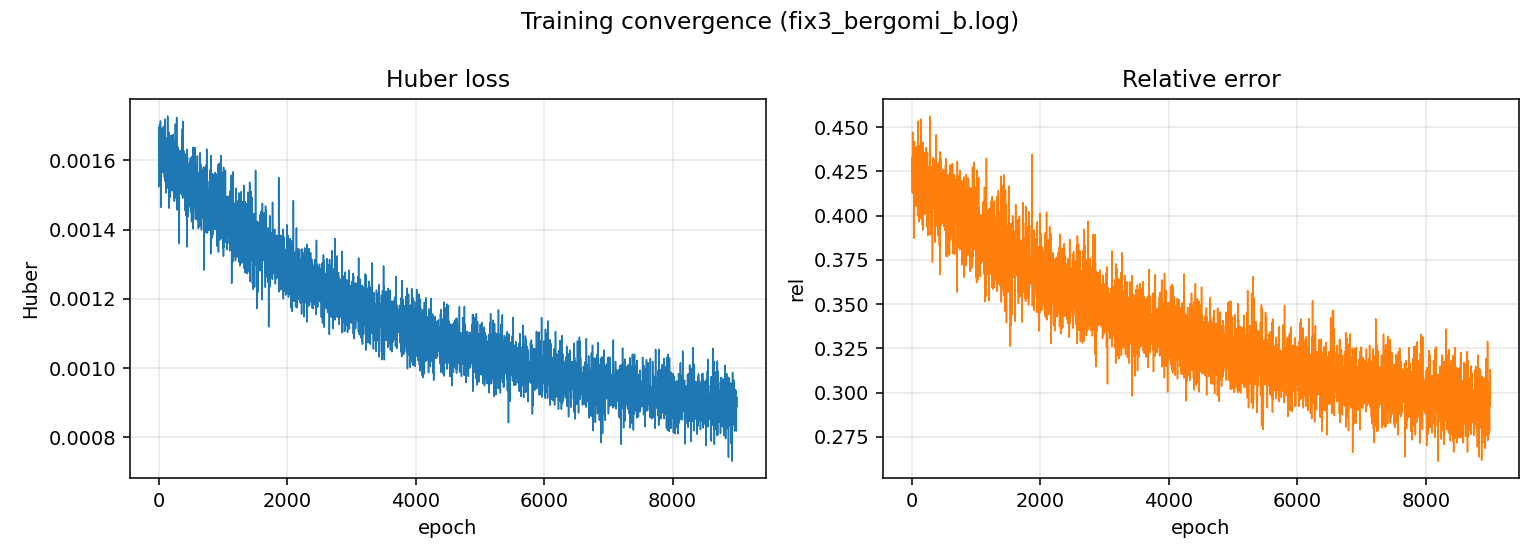
\includegraphics[width=\textwidth]{fig_convergence.png}
\caption{Training trajectory for a representative cell. Huber reconstruction
loss (left) and relative error (right) across fine-tuning epochs.}
\label{fig:convergence}
\end{figure}

\paragraph{A note on early stopping.} In the calmest regime (2013--2015), three
cells initially appeared to collapse at epoch~1 under a rule terminating after
10 consecutive non-improving epochs. This was a false positive: the
learning-rate scheduler does not engage until epoch~15, every cell in that
regime exhibits rising validation loss over the first 10--20 epochs, and a
surviving cell showed an identical early trajectory before descending to the
best loss in its regime. Relaxing the rule to 30 consecutive increases, armed
after epoch~20, recovered all three cells, which trained to epochs 717--744 with
12--21\% improvements over initialisation.

\subsection{Evaluation protocols}
\label{sec:protocols}

\paragraph{In-sample.} All cells are evaluated on the full regime, reporting
vega-weighted implied-volatility RMSE. Because the arms are separately estimated
rather than nested in the estimation sense, we use two-sided Diebold-Mariano
tests \citep{diebold1995} as the primary comparison; Clark-West statistics
\citep{clark2007} are computed but interpreted with caution.

All test statistics use a Newey-West HAC variance estimator \citep{newey1987}
with the automatic bandwidth rule of \citet{andrews1991},
$\lfloor 4(T/100)^{2/9}\rfloor$. Daily surface loss differentials are strongly
serially correlated, and unadjusted $t$-statistics would be materially inflated.

\paragraph{Walk-forward.} Within each regime the sample is split into quarterly
blocks. The model trains on all quarters up to $Q$ and is evaluated on $Q+1$,
rolling forward, warm-started from the previous window. This yields 36 windows
per model per arm.

\paragraph{Benchmarks.} Both arms are compared against a previous-day
persistence forecast and an at-the-money-flat surface, scored identically.
Section~\ref{sec:benchmark} additionally reports the comparison in normalised
price units and against a classical least-squares calibration.

\paragraph{Hedging.} For each cell we run a rolling at-the-money delta hedge
over every trading day, using 20{,}000 Monte Carlo paths, comparing the variance
of the hedging error between arms.

\paragraph{Multiple testing.} We report Benjamini-Hochberg
\citep{benjamini1995} adjusted $p$-values controlling the false discovery rate
at 5\%. All twelve nominally significant out-of-sample results survive. In-sample
eight of nine survive; the exception is rBergomi 2013--2015 (raw $p = 0.031$,
adjusted $p = 0.055$), which we do not count among our significant findings.

\section{Results}

\subsection{In-sample pricing}

\begin{table}[h]
\centering
\caption{In-sample vega-weighted IV RMSE and Diebold-Mariano tests. Positive $t$
favours sentiment. $\dagger$ marks cells surviving Benjamini-Hochberg correction
at FDR 5\%.}
\label{tab:insample}
\begin{tabular}{llrrrrl}
\toprule
Model & Regime & $n$ & RMSE (NS) & RMSE (S) & DM $t$ & BH \\
\midrule
Bates    & 2010--2012 & 744 & 0.04758 & 0.04774 & $-1.87$  & \\
Bates    & 2013--2015 & 727 & 0.06571 & 0.06554 & $1.64$   & \\
Bates    & 2016--2019 & 995 & 0.06033 & 0.06111 & $-6.89$  & $\dagger$ \\
Bates    & 2020--2022 & 749 & 0.06799 & 0.06773 & $1.72$   & \\
Bergomi  & 2010--2012 & 744 & 0.05123 & 0.05141 & $-0.96$  & \\
Bergomi  & 2013--2015 & 727 & 0.05430 & 0.05416 & $0.34$   & \\
Bergomi  & 2016--2019 & 995 & 0.05331 & 0.05216 & $4.01$   & $\dagger$ \\
Bergomi  & 2020--2022 & 749 & 0.07303 & 0.07889 & $-0.90$  & \\
Heston   & 2010--2012 & 744 & 0.05242 & 0.05004 & $12.46$  & $\dagger$ \\
Heston   & 2013--2015 & 727 & 0.04786 & 0.04850 & $-4.94$  & $\dagger$ \\
Heston   & 2016--2019 & 995 & 0.04746 & 0.04611 & $8.01$   & $\dagger$ \\
Heston   & 2020--2022 & 749 & 0.06957 & 0.06706 & $7.57$   & $\dagger$ \\
rBergomi & 2010--2012 & 744 & 0.06064 & 0.06002 & $0.81$   & \\
rBergomi & 2013--2015 & 727 & 0.05141 & 0.05044 & $2.16$   & \\
rBergomi & 2016--2019 & 995 & 0.04836 & 0.04635 & $7.37$   & $\dagger$ \\
rBergomi & 2020--2022 & 749 & 0.08111 & 0.08464 & $-3.57$  & $\dagger$ \\
\bottomrule
\end{tabular}
\end{table}

Eleven of sixteen cells show a nominally significant difference, split seven
favourable and four unfavourable; eight survive FDR control. Effect sizes are
uniformly small: the largest, Heston 2010--2012, is a 4.5\% RMSE reduction.
Heston benefits most consistently. The Bergomi family, which already imposes
flexible forward-variance dynamics, shows little consistent gain.

\begin{figure}[h]
\centering
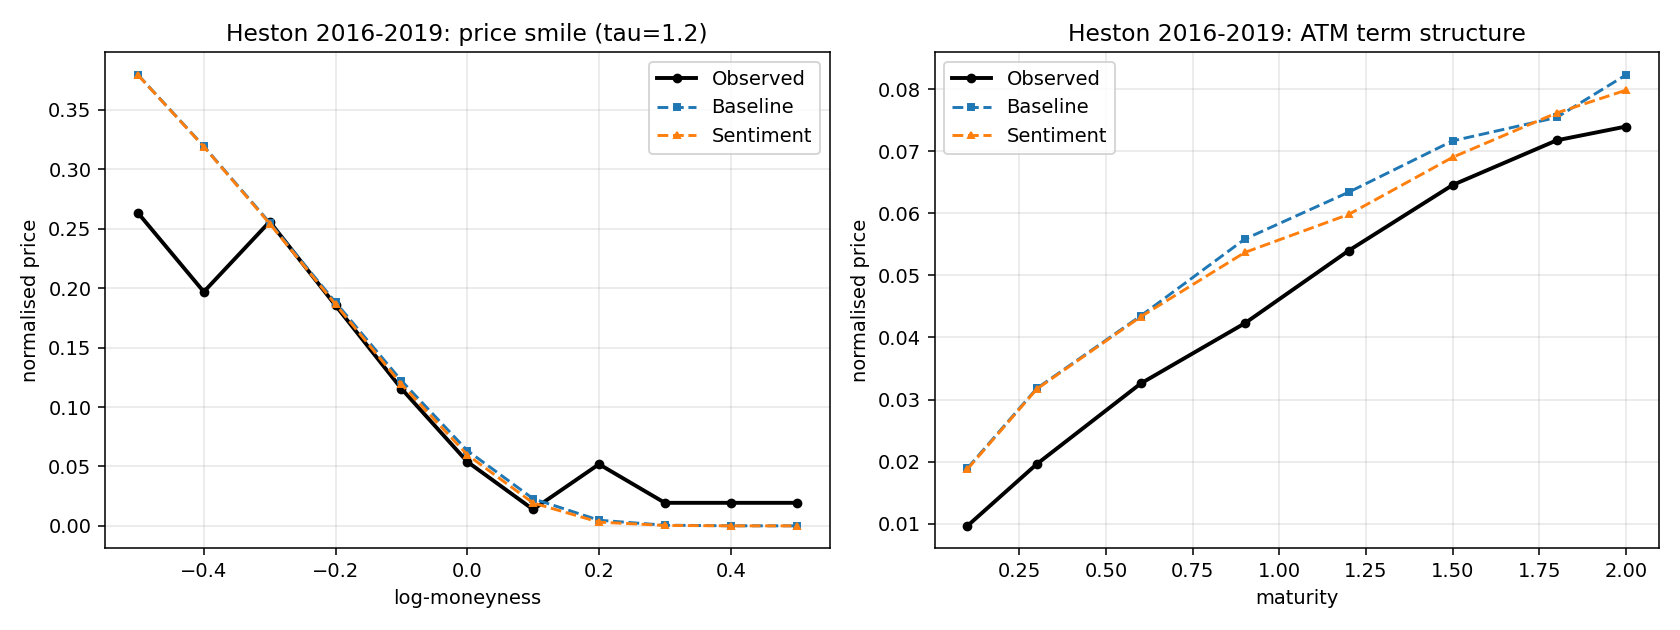
\includegraphics[width=\textwidth]{fig_smile_term_Heston_2016-2019.png}
\caption{Price smile at a representative maturity (left) and ATM term structure
(right) for Heston in 2016--2019, both arms against the observed market surface.}
\label{fig:smile}
\end{figure}

\begin{figure}[h]
\centering
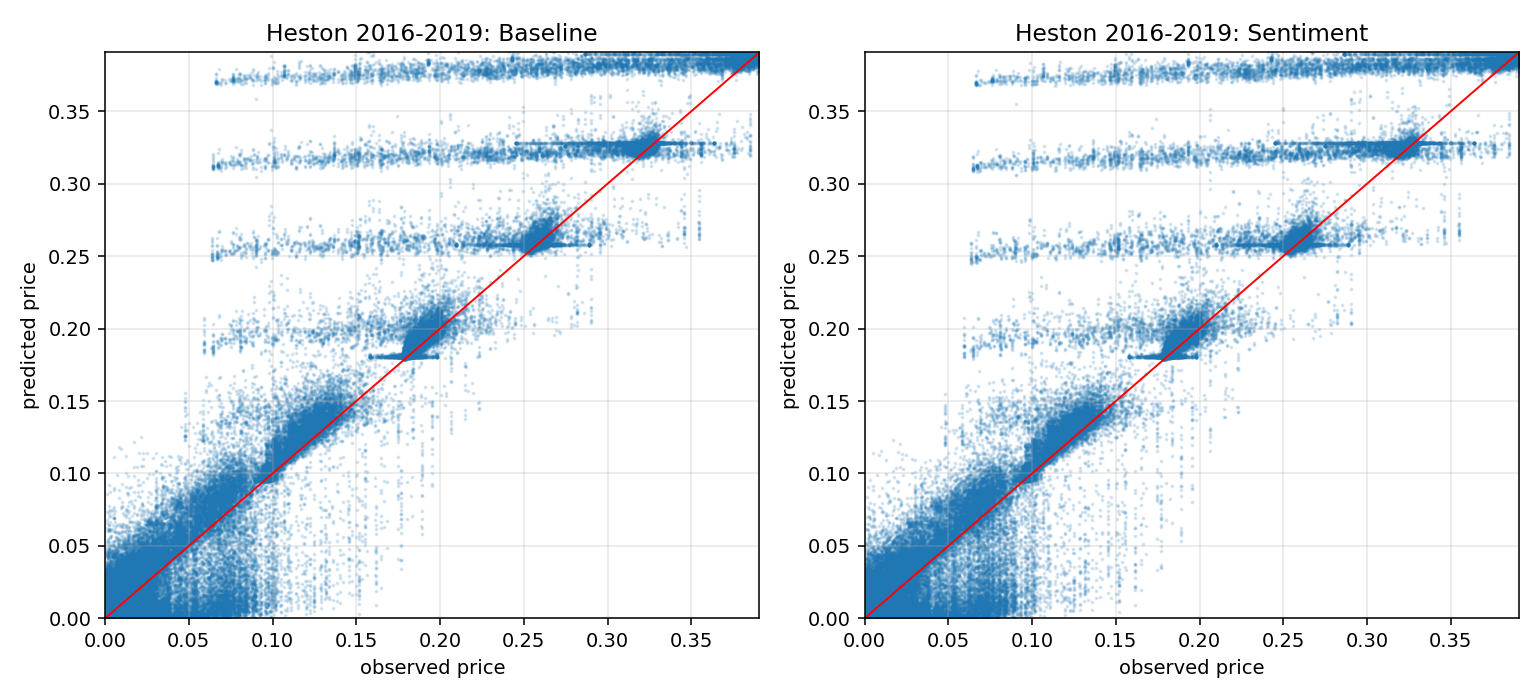
\includegraphics[width=0.9\textwidth]{fig_parity_Heston_2016-2019.png}
\caption{Predicted versus observed normalised prices, baseline (left) and
sentiment (right), Heston 2016--2019.}
\label{fig:parity}
\end{figure}

\begin{figure}[h]
\centering
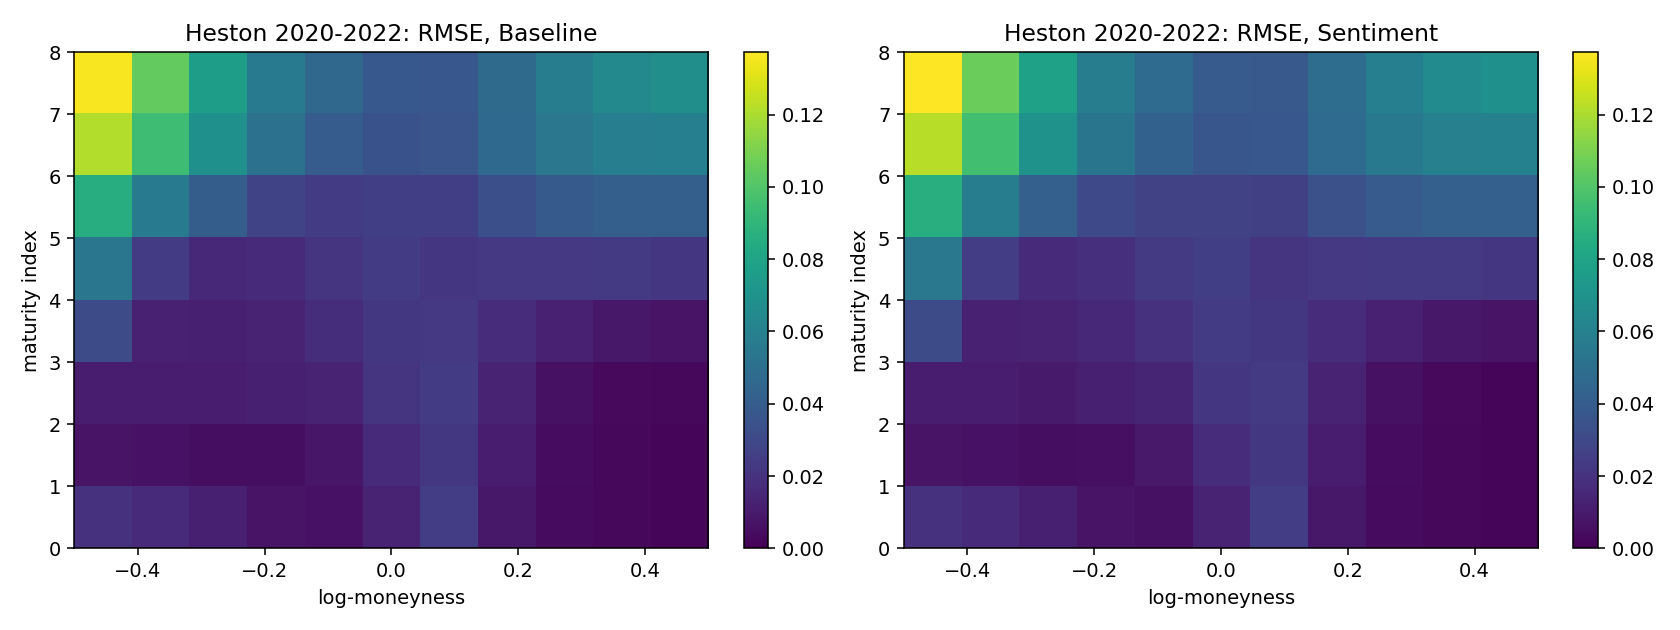
\includegraphics[width=\textwidth]{fig_error_heatmap_Heston_2020-2022.png}
\caption{Per-node RMSE across the $8\times11$ grid, both arms, Heston
2020--2022. Errors concentrate in the deepest out-of-the-money wings and at the
shortest maturities.}
\label{fig:heatmap}
\end{figure}

\subsection{Out-of-sample walk-forward}

\begin{table}[h]
\centering
\small
\caption{Walk-forward out-of-sample results, with in-sample comparison.
$\dagger$ marks cells surviving Benjamini-Hochberg correction at FDR 5\%.}
\label{tab:oos}
\begin{tabular}{llrrrrlrl}
\toprule
Model & Regime & $n$ & RMSE (NS) & RMSE (S) & OOS $t$ & BH & In-s.\ $t$ & Agree \\
\midrule
Bates    & 2010--2012 & 494 & 0.05735 & 0.05606 & $10.13$ & $\dagger$ & $-1.87$ & no \\
Bates    & 2013--2015 & 478 & 0.10152 & 0.10130 & $1.14$  &           & $1.64$  & yes \\
Bates    & 2016--2019 & 745 & 0.09470 & 0.09371 & $9.23$  & $\dagger$ & $-6.89$ & no \\
Bates    & 2020--2022 & 496 & 0.06217 & 0.06110 & $9.39$  & $\dagger$ & $1.72$  & yes \\
Bergomi  & 2010--2012 & 494 & 0.05606 & 0.05633 & $-2.15$ & $\dagger$ & $-0.96$ & yes \\
Bergomi  & 2013--2015 & 478 & 0.11608 & 0.11657 & $-2.40$ & $\dagger$ & $0.34$  & no \\
Bergomi  & 2016--2019 & 745 & 0.10329 & 0.10400 & $-2.92$ & $\dagger$ & $4.01$  & no \\
Bergomi  & 2020--2022 & 496 & 0.04357 & 0.04349 & $0.92$  &           & $-0.90$ & no \\
Heston   & 2010--2012 & 494 & 0.04629 & 0.04637 & $-0.44$ &           & $12.46$ & no \\
Heston   & 2013--2015 & 478 & 0.08369 & 0.08382 & $-0.95$ &           & $-4.94$ & yes \\
Heston   & 2016--2019 & 745 & 0.07014 & 0.06943 & $8.99$  & $\dagger$ & $8.01$  & yes \\
Heston   & 2020--2022 & 496 & 0.04215 & 0.04150 & $6.40$  & $\dagger$ & $7.57$  & yes \\
rBergomi & 2010--2012 & 494 & 0.08136 & 0.08197 & $-3.23$ & $\dagger$ & $0.81$  & no \\
rBergomi & 2013--2015 & 478 & 0.05837 & 0.05802 & $2.68$  & $\dagger$ & $2.16$  & yes \\
rBergomi & 2016--2019 & 745 & 0.05123 & 0.05146 & $-2.30$ & $\dagger$ & $7.37$  & no \\
rBergomi & 2020--2022 & 496 & 0.04417 & 0.04470 & $-4.96$ & $\dagger$ & $-3.57$ & yes \\
\bottomrule
\end{tabular}
\end{table}

Out-of-sample, seven cells favour sentiment significantly and six favour the
baseline; all twelve survive FDR control. The aggregate verdict is as equivocal
as in-sample---but the cell-level agreement is not. \textbf{The in-sample and
out-of-sample signs disagree in six of sixteen cells}:

\begin{itemize}
\item \textbf{Heston 2010--2012}, the largest in-sample advantage in the study
($t = 12.46$), is indistinguishable from zero out-of-sample ($t = -0.44$).
\item \textbf{Bates reverses direction entirely.} In-sample it is the family
sentiment appears to harm most; out-of-sample sentiment wins its three
significant cells decisively.
\item \textbf{Bergomi and rBergomi 2016--2019} flip from significantly
favourable in-sample to significantly unfavourable out-of-sample.
\end{itemize}

What survives with the same sign and significance in both protocols is a
minority: Heston in 2016--2019 and 2020--2022, rBergomi in 2013--2015, and Bates
in 2020--2022.

We regard this as the paper's central methodological finding. In-sample
surface-fit comparison is not a reliable guide to whether an additional input
channel carries transferable information; \citet{diebold2015} makes a related
point about the interpretation of predictive-accuracy tests.

The offline/online process mismatch corrected in
Appendix~\ref{app:corrections}~(A.7) affected Bates alone, and Bates is also the
family exhibiting the largest reversal. All results use the corrected generator;
we note the coincidence explicitly because Bates carried an additional
correction the other three families did not.

\subsection{Benchmark comparison and the sensitivity of the comparison to the
error metric}
\label{sec:benchmark}

Under the vega-weighted implied-volatility metric, a previous-day persistence
forecast attains lower error than every calibrated variant in all sixteen cells,
by a mean factor of 2.0 (Table~\ref{tab:benchmark}, left panel).

This result is metric-dependent, and materially so. Measured in normalised price
RMSE on the identical predictions and days, the same comparison yields a mean
ratio of \textbf{1.08}, ranging from 1.03 to 1.20.

\begin{table}[h]
\centering
\caption{Benchmark comparison under two error metrics. Persistence uses the
previous day's surface and is scored identically to the models. Model ranges
span the four families within each regime.}
\label{tab:benchmark}
\begin{tabular}{lrlrrlr}
\toprule
& \multicolumn{3}{c}{vega-weighted IV RMSE} & \multicolumn{3}{c}{normalised price RMSE} \\
\cmidrule(lr){2-4}\cmidrule(lr){5-7}
Regime & persist. & models & ratio & persist. & models & ratio \\
\midrule
2010--2012 & 0.0277 & 0.0480--0.0607 & 1.73--2.19 & 0.0489 & 0.0508--0.0529 & 1.04--1.08 \\
2013--2015 & 0.0231 & 0.0482--0.0656 & 2.09--2.84 & 0.0495 & 0.0555--0.0593 & 1.12--1.20 \\
2016--2019 & 0.0208 & 0.0464--0.0604 & 2.23--2.91 & 0.0425 & 0.0443--0.0470 & 1.04--1.11 \\
2020--2022 & 0.0589 & 0.0682--0.0818 & 1.16--1.39 & 0.0396 & 0.0407--0.0421 & 1.03--1.06 \\
\bottomrule
\end{tabular}
\end{table}

The mechanism is the vega weighting together with the price-to-IV inversion.
Converting a price error into an implied-volatility error divides by vega, so in
regions of small vega---the deep wings and shortest maturities, precisely where
parametric models fit worst---a modest price error becomes a large IV error.
Persistence is insulated because the IV surface is itself highly persistent
\citep{cont2002}.

We report both because the divergence is the substantive point: \textbf{the
choice of error metric determines whether a calibrated parametric model or a
random walk appears superior.} Neither number is incorrect. A desk pricing
options cares about price error; one managing vega exposure cares about IV
error. Studies in this literature routinely report one without the other.

\subsubsection{Is the residual error attributable to the neural calibration?}
A natural objection is that the persistence gap reflects an underfitting neural
calibration rather than a limitation of the model class. We test this by
calibrating the same pricer to the same surfaces by classical least squares
(trust-region reflective with box constraints on the Table~\ref{tab:bounds}
bounds, warm-started, 300 function evaluations per day) on 20 evenly-spaced days
per cell.

\begin{table}[h]
\centering
\caption{Neural versus classical calibration, Heston, normalised price RMSE.}
\label{tab:classical}
\begin{tabular}{lrrrr}
\toprule
Cell & classical (median) & classical (pooled) & network & persistence \\
\midrule
Heston 2016--2019 & 0.0418 & 0.0443 & 0.0444 & 0.0425 \\
Heston 2020--2022 & 0.0389 & 0.0438 & 0.0409 & 0.0396 \\
\bottomrule
\end{tabular}
\end{table}

Classical and neural calibration attain comparable surface fit. On typical days
the classical optimiser is marginally better, but its pooled error is equal or
worse, reflecting greater variability in per-day fit quality: it occasionally
converges poorly, whereas the network's single forward pass is more consistent.
Neither method closes the gap to persistence in price space. We accordingly
attribute the residual fitting error to the capacity of the parametric model
class, not to the calibration procedure.

\subsection{Delta-hedged profit and loss (H2)}
Across the sixteen cells, the sentiment arm attains lower hedging-error variance
in nine and higher in seven. More informative is the relationship to the pricing
result: \textbf{the hedging and in-sample pricing verdicts agree in twelve of
sixteen cells.} Hedging does not reveal a sentiment benefit invisible to
pricing.

The largest effects appear in the COVID regime: Heston 2020--2022 shows a 12.5\%
variance reduction and rBergomi 2020--2022 a 15.8\% reduction. The four
disagreements cluster in rBergomi, the family with the weakest parameter
identification.

\begin{figure}[h]
\centering
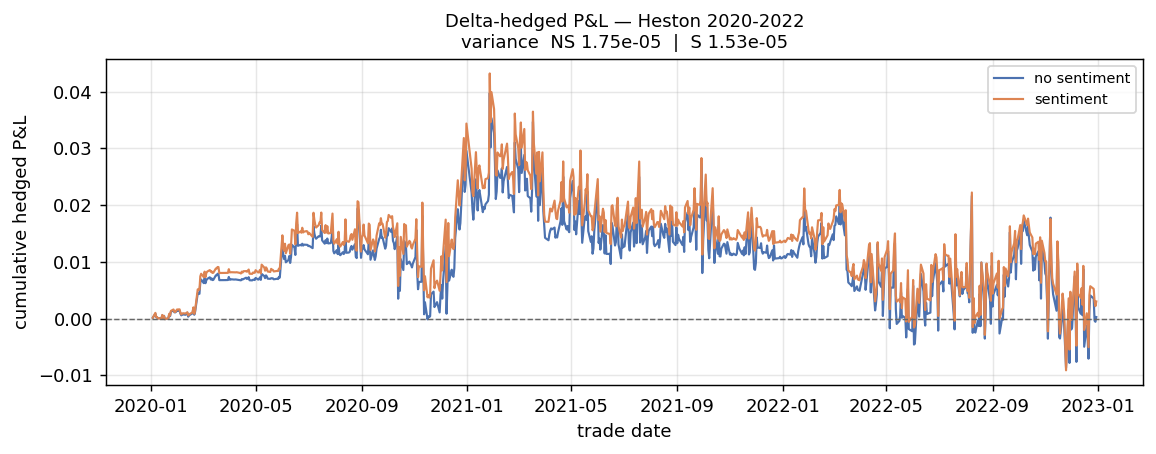
\includegraphics[width=0.85\textwidth]{hedge_Heston_2020-2022.png}
\caption{Delta-hedged P\&L for Heston 2020--2022, the cell with the largest
variance reduction attributable to sentiment ($-12.5\%$).}
\label{fig:hedge}
\end{figure}

H2 is not supported in general, with the qualified exception of specific
high-volatility cells.

\subsection{No-arbitrage diagnostics}
Butterfly violations are essentially absent (0.0000--0.0016). Calendar-spread
violations range from 1.4\% to 19\%, which at face value would concern models
that are martingale by construction.

A targeted diagnostic shows these are Monte Carlo noise. Violations concentrate
at the long end of the maturity axis---for a representative cell, the rate rises
monotonically from 0.000 in the $0.1\to0.3$ gap to 0.153 in the $1.8\to2.0$
gap---where the true increment in total variance is smallest and most easily
flipped by simulation error. The median violation magnitude is 0.00311 against a
median positive increment of 0.00812, a ratio of 0.38. Real pathology would
concentrate at the short end and survive a generous tolerance; neither holds.

\subsection{Parameter identification}
\label{sec:ident}
We assess identification using the ratio of the standard deviation of observed
daily parameter changes to that arising if the parameter were redrawn uniformly
from its Table~\ref{tab:bounds} bounds each day. A ratio near 1 indicates the
network is effectively guessing.

Mean-reversion speed has ratios of 1.0--1.2 in nearly every cell: the network's
day-to-day variation in $\kappa$ is as large as drawing uniformly from
$[0.1, 3.0]$ afresh each day. Long-run and initial variance frequently exceed
0.9. The best-identified parameters are vol-of-vol, correlation and the jump
parameters, at 0.4--0.6.

Critically, \textbf{the sentiment and baseline arms have nearly identical ratios
in every row}, differing only in the third decimal. Calibrated parameter values
from this pipeline should not be interpreted as estimates of physical
quantities.

\section{Discussion}

\subsection{On H1}
H1 is not supported in the form stated. Sentiment does not produce a general
reduction in pricing error, and the regime prediction is wrong: gains are not
concentrated in high-volatility periods. The defensible statement is
conditional---sentiment produces small, model-dependent effects robust to
out-of-sample validation in a minority of cells.

\subsection{Why offline gains do not transfer}
The network demonstrably can extract information from a sentiment channel
(Table~\ref{tab:offline}). What differs online is the channel itself.

The synthetic channel omits the dominant term of the empirical sentiment
process. As Table~\ref{tab:regression} shows, real sentiment is overwhelmingly
autoregressive ($t = 58.6$), and that term cannot be reproduced on a simulated
path. The offline network learns to exploit a return-driven signal and then
meets an online signal whose principal component is persistence it has never
seen.

Note that the offline channel is not merely redundant with the surface. Because
the synthetic surfaces are generated by dynamics in which a latent sentiment
process causally drives variance (Section~\ref{sec:synthsent}), a genuine
sentiment--volatility relationship exists for the network to learn. The failure
of transfer is more plausibly about the \emph{form} of the observed signal than
about the absence of an underlying relationship.

\subsection{On benchmarks and metrics}
Under the IV metric a random walk dominates every calibrated variant; under a
price metric the same predictions differ by 8\% on average, and a converged
classical optimiser performs no better than the network. What the comparison
establishes is that claims about surface accuracy should be accompanied by a
random-walk comparison and an explicit statement of metric.

\section{Limitations}
\begin{description}
\item[Sentiment representation.] A single daily scalar. Topic-conditioned
scores, intraday timing or source diversification might carry information this
aggregation destroys.
\item[The synthetic sentiment gap.] The generator substitutes a return-based
proxy for the lagged-sentiment term that dominates the empirical fit.
\item[Parameter identification.] Most structural parameters are weakly
identified; the calibrated parameters carry little interpretive weight.
\item[Classical benchmark configuration.] Warm-started across days, 20 days per
cell. It establishes comparability but is not an exhaustive benchmark; the
identification diagnostics from those runs reflect the warm start and are not
reported.
\item[Residual synthetic-data floor.] 0.22--0.70\% of synthetic surface points
remain at the inversion floor, confined to regions where vega is negligible.
\item[Scope.] Four families, four regimes, one index, one sentiment source, 750
fine-tuning epochs, 20 refit epochs per walk-forward window.
\item[Multiple comparisons.] We report Benjamini-Hochberg adjusted $p$-values
throughout; all twelve out-of-sample and eight of nine in-sample nominally
significant results survive FDR control at 5\%. We report every cell and have
not selected a subset post hoc.
\end{description}

\section{Conclusion}
We set out to test whether financial-news sentiment improves neural-SDE option
pricing, expecting the clearest benefits in volatile markets. After rebuilding
the pipeline to correct seven data-generation defects, training 32 cells, and
evaluating under both in-sample and expanding-window walk-forward protocols, we
find that it does not, in the general form hypothesised.

What we find instead is more specific. The sentiment channel is learnable in
principle---it improves offline validation loss in all four families. Online, it
produces small and heterogeneous effects surviving out-of-sample validation in
only a minority of cells. In-sample and out-of-sample evaluation disagree in six
of sixteen cells, including a complete reversal for one family and the
disappearance of the study's largest in-sample effect.

Every model variant is outperformed by a previous-day persistence forecast under
the vega-weighted IV metric---though by only 8\% on average in price units, and a
converged classical calibration performs no better than the network. The
apparent dominance of the naive benchmark is largely an artifact of how surface
error is measured.

The methodological conclusions are the ones we would most want carried forward:
that in-sample surface comparison is insufficient to establish that an auxiliary
input carries transferable information; that a random-walk benchmark and an
explicit statement of error metric belong alongside any reported surface RMSE;
and that calibrated parameters from a deep-calibration pipeline should not be
read as identified estimates without an explicit identification check.

\appendix
\section{Corrections to the offline data-generation stage}
\label{app:corrections}

An earlier iteration produced qualitatively different conclusions---most notably
that sentiment helped most in the calmest regime. That finding did not survive
correction of the following defects.

\paragraph{A.1 Martingale defect.} Terminal simulated prices did not satisfy
$\mathbb{E}[S_T] = F$. The discretised variance process under naive clamping
produced a drift error reaching $-19\%$ at $T = 2$. Corrected by rescaling $S_T$
by its sample mean at every pricing site.

\paragraph{A.2 Variance discretisation.} Naive clamping was replaced with full
truncation \citep{lord2010}.

\paragraph{A.3 Quadrature weights.} Gauss-Laguerre weights were constructed by a
manual recursion subject to catastrophic cancellation, producing a maximum
relative weight error of 6.6\%. Replaced with a standard library implementation.

\paragraph{A.4 Sentiment channel axis error.} The synthetic sentiment channel
was written by indexing the Monte Carlo \emph{path} axis rather than
broadcasting across strikes. The resulting channel contained eleven unrelated
path draws presented as a strike profile---noise structured to look like a
signal. After correction the channel is constant across strikes within a
maturity slice, with adjacent-maturity correlations of $+0.74$ to $+0.89$.

\paragraph{A.5 Strike grid.} Synthetic surfaces were built on a linear strike
grid while market surfaces used log-moneyness. Unified to log-moneyness on
$[-0.5, +0.5]$.

\paragraph{A.6 Regression coefficients.} The generator applied a superseded
coefficient set whose return and volatility loadings were 5.6--7.1 times those
of the current fit. Replaced with the coefficients in
Table~\ref{tab:regression}.

\paragraph{A.7 Jump compensator.} The offline generator omitted the Merton jump
compensator, $\lambda_J(e^{\mu_J + \sigma_J^2/2} - 1)$, from the log-price
drift, while the online differentiable pricer subtracted it. The two stages
therefore simulated different Bates processes: the offline surfaces carried an
uncompensated drift, so the network was pre-trained on a mapping that did not
correspond to the model it was later asked to calibrate. Corrected by
subtracting the compensator in the generator's drift term.

\paragraph{Effect of the corrections.} The inversion-failure rate fell from
16.8--37.6\% to 0.22--0.70\%. The offline sentiment-arm advantage fell from
6--42\% to 4--25\%, indicating that part of the apparent offline benefit came
from the inflated variance of the corrupted channel. The earlier finding that
sentiment helps most in 2013--2015 disappeared entirely.

We document these in full because the corrected and uncorrected pipelines
support opposite conclusions, and because several defects (A.1, A.2, A.4) would
be invisible in aggregate loss curves. Training-loss diagnostics alone were not
sufficient to detect any of them.

\begin{thebibliography}{99}

\bibitem[Andrews(1991)]{andrews1991}
Andrews, D.~W.~K. (1991). Heteroskedasticity and autocorrelation consistent
covariance matrix estimation. \emph{Econometrica}, 59(3), 817--858.

\bibitem[Araci(2019)]{araci2019}
Araci, D. (2019). FinBERT: financial sentiment analysis with pre-trained
language models. arXiv:1908.10063.

\bibitem[Baker and Wurgler(2006)]{baker2006}
Baker, M. and Wurgler, J. (2006). Investor sentiment and the cross-section of
stock returns. \emph{The Journal of Finance}, 61(4), 1645--1680.

\bibitem[Bakshi et al.(1997)]{bakshi1997}
Bakshi, G., Cao, C. and Chen, Z. (1997). Empirical performance of alternative
option pricing models. \emph{The Journal of Finance}, 52(5), 2003--2049.

\bibitem[Bates(1996)]{bates1996}
Bates, D.~S. (1996). Jumps and stochastic volatility: exchange rate processes
implicit in Deutsche Mark options. \emph{The Review of Financial Studies}, 9(1),
69--107.

\bibitem[Bayer et al.(2016)]{bayer2016}
Bayer, C., Friz, P. and Gatheral, J. (2016). Pricing under rough volatility.
\emph{Quantitative Finance}, 16(6), 887--904.

\bibitem[Bayer and Stemper(2018)]{bayer2018}
Bayer, C. and Stemper, B. (2018). Deep calibration of rough stochastic
volatility models. arXiv:1810.03399.

\bibitem[Benjamini and Hochberg(1995)]{benjamini1995}
Benjamini, Y. and Hochberg, Y. (1995). Controlling the false discovery rate: a
practical and powerful approach to multiple testing. \emph{Journal of the Royal
Statistical Society: Series B}, 57(1), 289--300.

\bibitem[Bergomi(2005)]{bergomi2005}
Bergomi, L. (2005). Smile dynamics II. \emph{Risk}, October 2005.

\bibitem[Carr and Madan(1999)]{carr1999}
Carr, P. and Madan, D. (1999). Option valuation using the fast Fourier
transform. \emph{Journal of Computational Finance}, 2(4), 61--73.

\bibitem[Clark and West(2007)]{clark2007}
Clark, T.~E. and West, K.~D. (2007). Approximately normal tests for equal
predictive accuracy in nested models. \emph{Journal of Econometrics}, 138(1),
291--311.

\bibitem[Cont and da Fonseca(2002)]{cont2002}
Cont, R. and da Fonseca, J. (2002). Dynamics of implied volatility surfaces.
\emph{Quantitative Finance}, 2(1), 45--60.

\bibitem[Devlin et al.(2019)]{devlin2019}
Devlin, J., Chang, M.-W., Lee, K. and Toutanova, K. (2019). BERT: pre-training
of deep bidirectional transformers for language understanding. \emph{Proceedings
of NAACL-HLT 2019}, 4171--4186.

\bibitem[Diebold(2015)]{diebold2015}
Diebold, F.~X. (2015). Comparing predictive accuracy, twenty years later.
\emph{Journal of Business \& Economic Statistics}, 33(1), 1--9.

\bibitem[Diebold and Mariano(1995)]{diebold1995}
Diebold, F.~X. and Mariano, R.~S. (1995). Comparing predictive accuracy.
\emph{Journal of Business \& Economic Statistics}, 13(3), 253--263.

\bibitem[Ferguson and Green(2018)]{ferguson2018}
Ferguson, R. and Green, A. (2018). Deeply learning derivatives.
arXiv:1809.02233.

\bibitem[Gatheral et al.(2018)]{gatheral2018}
Gatheral, J., Jaisson, T. and Rosenbaum, M. (2018). Volatility is rough.
\emph{Quantitative Finance}, 18(6), 933--949.

\bibitem[Giacomini and White(2006)]{giacomini2006}
Giacomini, R. and White, H. (2006). Tests of conditional predictive ability.
\emph{Econometrica}, 74(6), 1545--1578.

\bibitem[Gon\c{c}alves and Guidolin(2006)]{goncalves2006}
Gon\c{c}alves, S. and Guidolin, M. (2006). Predictable dynamics in the S\&P 500
index options implied volatility surface. \emph{The Journal of Business}, 79(3),
1591--1635.

\bibitem[Heston(1993)]{heston1993}
Heston, S.~L. (1993). A closed-form solution for options with stochastic
volatility with applications to bond and currency options. \emph{The Review of
Financial Studies}, 6(2), 327--343.

\bibitem[Horvath et al.(2021)]{horvath2021}
Horvath, B., Muguruza, A. and Tomas, M. (2021). Deep learning volatility: a deep
neural network perspective on pricing and calibration in (rough) volatility
models. \emph{Quantitative Finance}, 21(1), 11--27.

\bibitem[Hutchinson et al.(1994)]{hutchinson1994}
Hutchinson, J.~M., Lo, A.~W. and Poggio, T. (1994). A nonparametric approach to
pricing and hedging derivative securities via learning networks. \emph{The
Journal of Finance}, 49(3), 851--889.

\bibitem[Lord et al.(2010)]{lord2010}
Lord, R., Koekkoek, R. and van Dijk, D. (2010). A comparison of biased
simulation schemes for stochastic volatility models. \emph{Quantitative
Finance}, 10(2), 177--194.

\bibitem[Loughran and McDonald(2011)]{loughran2011}
Loughran, T. and McDonald, B. (2011). When is a liability not a liability?
Textual analysis, dictionaries, and 10-Ks. \emph{The Journal of Finance}, 66(1),
35--65.

\bibitem[Newey and West(1987)]{newey1987}
Newey, W.~K. and West, K.~D. (1987). A simple, positive semi-definite,
heteroskedasticity and autocorrelation consistent covariance matrix.
\emph{Econometrica}, 55(3), 703--708.

\bibitem[Tetlock(2007)]{tetlock2007}
Tetlock, P.~C. (2007). Giving content to investor sentiment: the role of media
in the stock market. \emph{The Journal of Finance}, 62(3), 1139--1168.

\end{thebibliography}

\end{document}
